The drilling operation will be controlled by a programmable logic controller (PLC) which will receive analog input from downhole and surface sensors, digitalize the data so that the control algorithm can be applied, and then transmit analog signals to the motor controllers to adjust the control parameters. The PLC can be programmed using Simulink which is integrated in Matlab, enabling the incorporation of Matlab algorithms. 

\numberwithin{equation}{section}
\numberwithin{figure}{section}
\numberwithin{table}{section}

The sensors included in the control system measure key drilling parameters. Vibration, inclination, azimuth and bit temperature will be monitored downhole, while RPM, torque, pressure, flow and the position of the ball screw are all surface measurements. The measurements will continuously be transmitted to and processed by the PLC which will in turn send signals to the hoisting motor, top drive and pump to adjust the WOP, RPM and flow rate.

\begin{figure} [H]
\centering
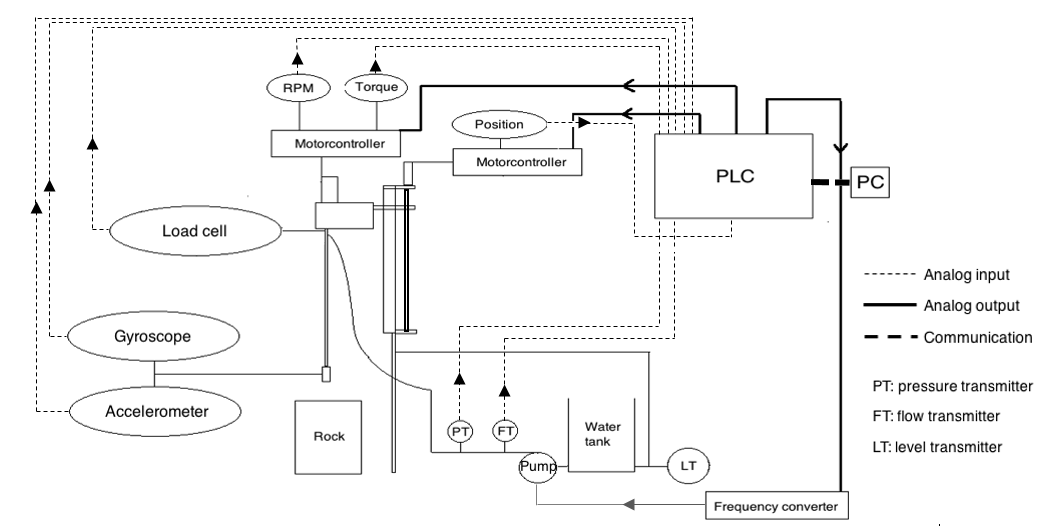
\includegraphics[width=1.0\textwidth]{figures/controlsystemflc.png}
\caption{Control System Flow Chart}
\label{fig:controlsystemflc}
\end{figure}

\subsection{Measurement and Sensors}

The analog data from the sensors will be transmitted to the PLC through wires. The wires will be placed inside the drill pipe, along the pipe wall. Wireless transmission was considered, but the water in the drill pipe, the thickness of the pipe wall and the rotation of the string, may cause noise which makes the data unreliable. 

No sensor is perfect, and even sensors from the same manufacturer can yield different readings. In addition to this, the sensors may change response if they are subjected to varying conditions like heat, humidity and shocks. Calibrating the sensors will therefore be of great importance to build and operate a complete automated drilling system. 

There are different methods of calibration, all varying in complexity \cite{ada}. The one-point method is the simplest method and is used when the sensor calibration is scaled and only sensor offset needs to be corrected. It is done by taking a measurement with the sensors, comparing the measurement with the reference standard, calculating the offset by subtracting the sensor reading from the reference reading and finally adding the offset to every sensor reading in the code.

The second method is two-point calibration. It is more complex than the one-point method, but can be applied to both scaled and raw sensor output. This method rescales the output and corrects both slope and offset errors. It can be used in cases where the output is known to be relatively linear. This method of calibration is performed by taking two measurements from the sensor: one near the low end and one near the high end. These measurements must then be repeated with the reference instrument and the corrected value can then be calculated by using equation (\ref{eq:twopoint})


\begin{equation}
\centering
   Corrected value = \frac{(raw Value - Raw Low Value) x Reference Range}{Raw Range}+Reference Low Value
\label{eq:twopoint}
\end{equation}

The last method is the multi-point curve fitting calibration. This is the most complex method and is used for sensors that are not linear. This can be done using Excel or similar spreadsheet programs. 

The need for calibration will be different for every sensor. The downhole sensors may experience large changes in conditions while the surface sensors will not, and they will therefore require a different type of calibration. 

Calibration will be performed during the testing period to determine reference standards for all sensors. Additional calibration will need to be done while drilling in case the sensor response changes. 

\subsubsection{Direct Output from Motors}
The RPM and the torque are direct outputs from the top drive motor. 
ROP will be estimated from the direct position output of the hoisting motor.

\subsubsection{Surface Sensors}
The following sensors are the sensors that will make measurements at surface. Some of these measurements will approximate downhole measurements.

\paragraph{Load Cell}
A load cell is a transducer which converts force into a measurable electrical output. It measures the tension in the drill string at surface, but the WOB can be estimated by suspending the bit off bottom. As the bit is lowered and touches bottom, the hook load decreases by an amount equal to the WOB. It will be placed at the top of the drill string.

\paragraph{Pressure Transducer}
A pressure transducer converts pressure into an analogue electrical signal. The main benefit of including this sensor is to be able to estimate the pressure in the different components of the circulation system.

\paragraph{Flowmeter}
A flowmeter is an instrument that measures the volumetric flow rate of a fluid, in this case the flow rate of the drilling fluid out of the pump. Because the pump pressure is expected to be high, the use of a flowmeter must be re-evaluated during the test phase. If the flowmeter cannot be used, the flow rate can be estimated from the rotational speed and cylinder size of the piston pump.

\subsubsection{Downhole Sensors}
\paragraph{Accelerometer and Gyroscope}
The accelerometer and the gyroscope will be included in the same sensor in the BHA. It will be placed over the constriction.

The accelerometer measures vibration, or acceleration, in the BHA. Its main use will be monitoring the amplitude of the vibrations.

The gyroscope provides estimates of inclination and azimuth by measuring the angle of deflection from the vertical. As the verticality of the borehole is an important factor during the competition, this will be a valuable measurement.

Temperature will also be measured using this sensor. The purpose of measuring the temperature is to avoid overheating the bit which can reduce the efficiency of drilling and damage the bit itself.

\subsection{Response Time}
The response time of measurements, data aggregation and control algorithms, will be estimated to ensure real-time control of the drilling process.

The response time of sensors will be determined experimentally as the theoretical approach requires thorough knowledge of the design of the sensor, its construction details, the properties and geometries of the sensor’s internal material as well as knowledge of the properties of the medium surrounding the sensor \cite{hash}.

Data aggregation will in this case consist of processing the data in the PLC and transmitting it to the PC.

Finally, the response time of the control algorithm needs to be estimated.